\section{Implementation and Calibration Details of \methodtitle{}}
\label{app:method-details}

\begin{figure}[t]
    \centering
    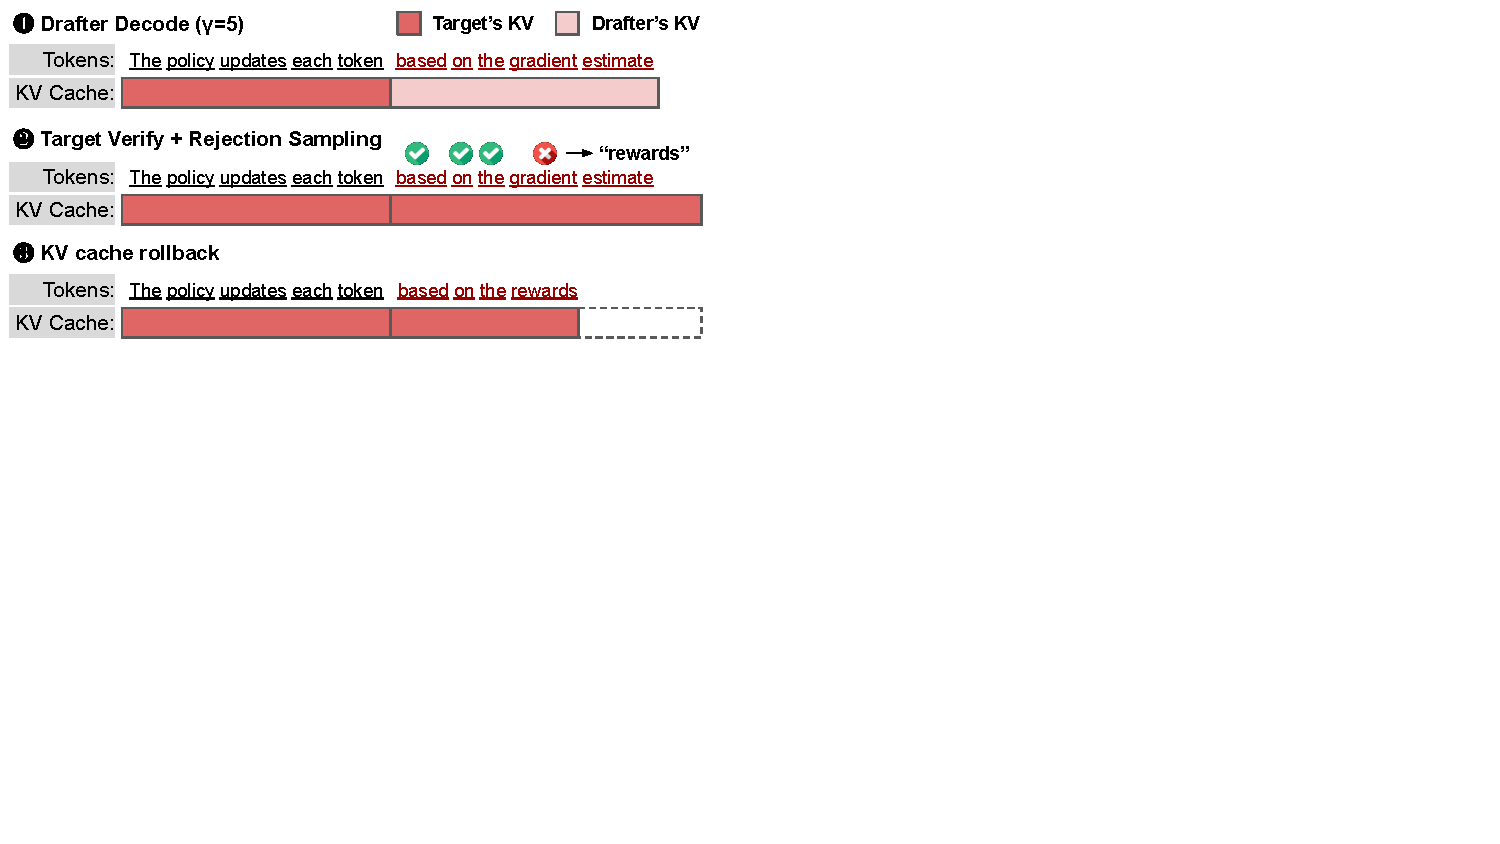
\includegraphics[width=0.6\linewidth]{figures/appendix_share_kv.pdf}
    \caption{
    Quantized self-SD with shared KV cache, target verification via rejection sampling, and rollback of rejected KV cache.
    }
    \label{fig:appendix_shared_kv}
\end{figure}

\subsection{KV-Cache Sharing between the Quantized Drafter and Target}
\label{app:shared-kv-sd}

\Cref{fig:appendix_shared_kv} illustrates the shared-KV execution pipeline used by \methodtitle{}.
The quantized drafter shares the target model's KV-cache storage, so drafting does not require an additional KV cache for the draft model.
At the start of each SD iteration, the prefix KV cache consists only of clean states produced by the full-precision target model.
The W4 drafter then proposes $\gamma$ tokens using quantized weights and writes provisional KV states for the drafted positions into the shared KV cache.

The target model verifies the drafted tokens in parallel using full-precision weights.
During verification, the target overwrites the provisional KV entries at the verified positions with clean target-generated KV states and performs rejection sampling to preserve the target-model sampling distribution.
If all drafted tokens are accepted, the target additionally samples the bonus token and the next SD iteration continues from the updated clean KV cache.
If a drafted token is rejected, the target resamples at the first rejected position from the adjusted target distribution, and all KV states after that position are discarded.
Thus, every new SD iteration begins from a prefix whose KV states are generated by the full-precision target model.

This design has two practical advantages for RL rollouts.
First, sharing the KV cache avoids the memory overhead of maintaining a separate drafter KV cache, which is important when rollout generation uses long maximum response lengths.
Second, because the drafter is reconstructed by quantizing the current target model at each training step, it remains synchronized with the evolving RL policy without auxiliary drafter training or online adaptation.

\subsection{Roofline-Based SD Toggle Model and Calibration}
\label{app:toggle_calibration}

We provide additional details on the parameters used in the SD toggle model and on the calibration procedure.

\paragraph{Parameter details.}
$W_T$ denotes the weight size of the target model in bytes, and $W_D$ denotes the weight size of the W4 drafter in bytes.
Because only the FFN and QKVO projection layers are quantized to 4 bits, while the embedding layer, LM head, and normalization layers remain in higher precision, the ratio $W_D/W_T$ is not exactly $25\%$; in practice, it is about $33$--$36\%$ of the original model size.
$C_{\mathrm{dense}}$ is the per-token dense compute cost, including FFN, QKVO projection, and LM-head computation, and $C_{\mathrm{attn}}$ is the per-token attention compute cost.
These quantities can be determined statically by the model architecture.

The effective per-token KV-cache traffic is modeled as
\[
\kappa_{\mathrm{eff}} = \rho_{\kappa}\,\kappa_{\mathrm{theoretical}},
\]
where $\kappa_{\mathrm{theoretical}}$ is the theoretical KV traffic determined by the model configuration,
\[
\kappa_{\mathrm{theoretical}}
=
(\#\mathrm{layers})
\times 2
\times (\#\mathrm{KV\ heads})
\times (\mathrm{head\ dim})
\times 2~\mathrm{bytes},
\]
with the factor of $2$ for key/value tensors and the final $2$ bytes corresponding to FP16 precision.
This quantity can be computed statically from the model architecture.
The scaling factor $\rho_{\kappa}$ is typically smaller than $1$, reflecting effects such as cache reuse and overlap with other operations.

The factor $\eta_D$ captures the practical overhead of W4A16 drafting.
Although weight quantization reduces the raw model weight size substantially, this does not translate directly into proportional memory-time reduction, because quantized decoding still incurs additional costs such as on-the-fly dequantization and kernel-level overhead.
Thus, $\eta_D$ models the aggregate overhead beyond the idealized weight-byte reduction.

Finally, we model the residual overhead terms as $c_T B$, $c_D B$, and $c_V B$ for target decoding, drafter decoding, and verification, respectively.
Empirically, we found that these residual overheads are dominated by batch-dependent effects, making a linear-in-batch approximation sufficiently accurate.

Our current formulation focuses on the TP$=1$ setting.
In principle, it can be generalized to TP$>1$ by augmenting each latency term with an explicit communication-overhead component, e.g., an all-reduce cost $c_{\mathrm{comm}}$.
We leave this extension to future work.

\paragraph{Calibration procedure.}
We calibrate the model in three stages.

First, we measure the effective compute throughput $\mathrm{F}_{\mathrm{eff}}$ using a hardware-specific microbenchmark based on repeated dense matrix multiplications.
Second, for each model of interest, we sweep full-precision target decoding, verification, and W4 quantized drafter decoding over a range of batch sizes and sequence lengths, with draft lengths $\gamma \in \{3, 7, 11, 15\}$.
Third, we fit the remaining parameters in two steps.
We first fit $\mathrm{BW}_{\mathrm{eff}}$, $\rho_{\kappa}$, and $c_T$ jointly using the target-model sweep data, and then fix them.
We next fit $\eta_D$, $c_D$, and $c_V$ using the drafter and verification sweep data.
Because self-SD uses the same architecture for the target and drafter, the compute term $C(B,S)$ is shared between target decoding and drafter decoding.
All fitted parameters are independent of $\gamma$; the dependence on draft length enters only through the verification compute term and the speedup model in \cref{eq:sd_speedup}.
This allows a model calibrated with a small set of draft lengths to generalize across other draft lengths without re-calibration.

In principle, $\mathrm{BW}_{\mathrm{eff}}$ should depend only on the hardware platform.
However, unlike $\mathrm{F}_{\mathrm{eff}}$, it is difficult to benchmark memory bandwidth in a directly comparable standalone form for our decoding workloads.
We therefore fit $\mathrm{BW}_{\mathrm{eff}}$ separately for each model.
In practice, the fitted values are consistent across models, typically falling in the range of 1560--1620~GB/s.

\begin{figure*}[t]
    \centering
    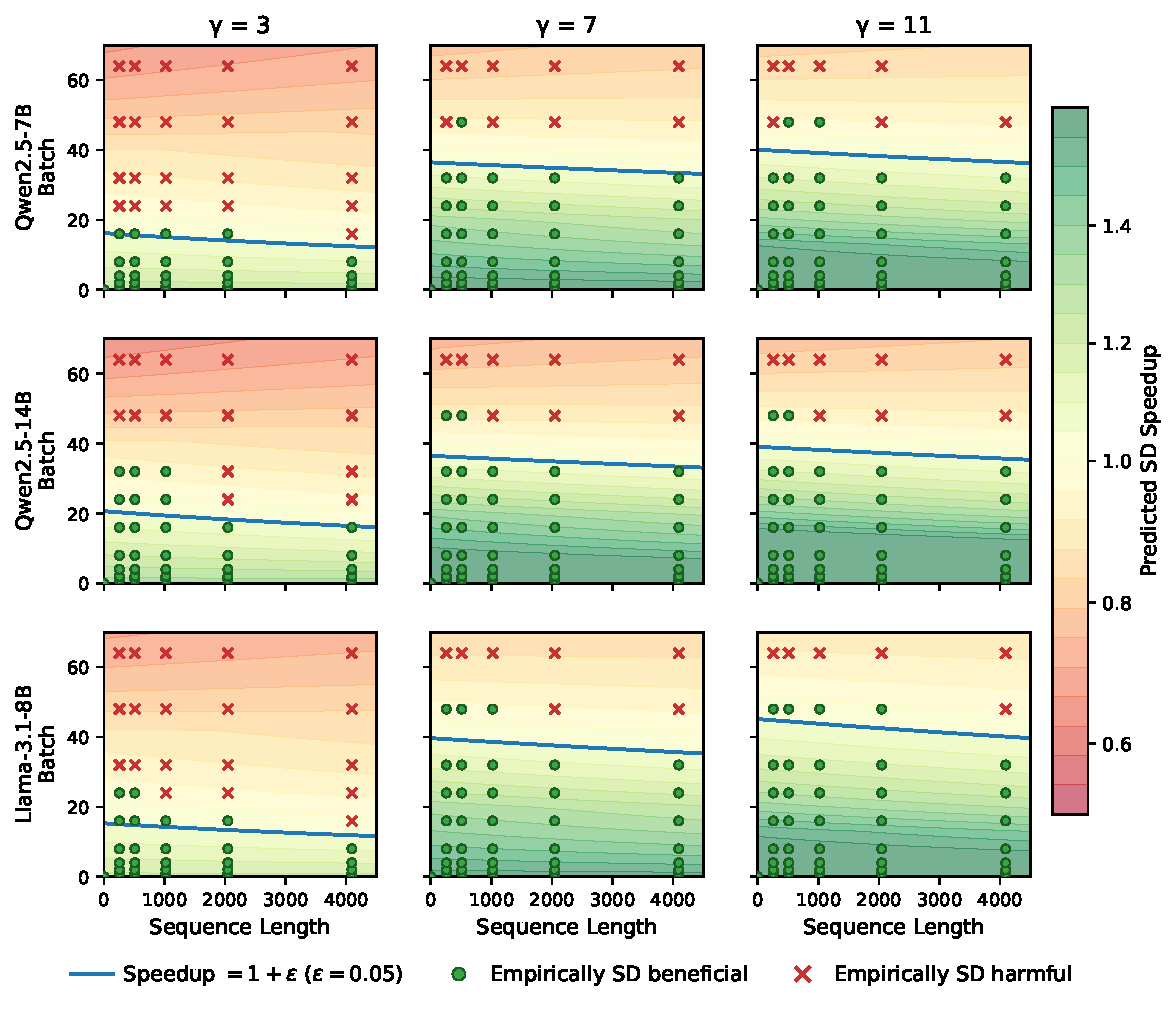
\includegraphics[width=0.8\textwidth]{figures/appendix_sd_grid.pdf}
    \caption{
    Validation of the roofline-based SD toggle policy.
    Background colors show predicted speedup, the blue line marks $\mathrm{Speedup}_{\mathrm{SD}}=1+\epsilon$, and markers indicate empirical SD-beneficial/harmful points.
    }
    \label{fig:appendix_sd_grid}
\end{figure*}

\subsection{Validation of the Roofline-Based SD Toggle Boundary}
\label{app:toggle_validation}

We validate the calibrated roofline model used by the SD toggle policy against measured W4 self-SD component timings.
For each model, we sweep active batch size $B$, sequence length $S$, and draft length $\DraftLength$, and measure the target decode time $\TargetTimebs$, quantized-drafter decode time $\DraftTimebs$, and target verification time $\VerifyTimebsg$ on a single A100 GPU with TP$=1$.
Using these measured components, we compute the empirical SD speedup using the same notation as~\cref{eq:sd_speedup}:
\begin{equation}
\mathrm{Speedup}_{\mathrm{emp}}(B,S,\gamma)
=
\frac{\mal \TargetTimebs}
{\DraftLength \DraftTimebs + \VerifyTimebsg}.
\label{eq:empirical_sd_speedup}
\end{equation}
For this validation, we use the optimistic setting $\mal=\DraftLength$, corresponding to full draft acceptance, to isolate the cost-model accuracy from block-efficiency variation.

\Cref{fig:appendix_sd_grid} compares the policy-predicted speedup surface with empirical measurements.
The background color shows the speedup predicted by the calibrated roofline model, and the blue contour indicates the toggle boundary at $\mathrm{Speedup}_{\mathrm{SD}}=1+\epsilon$ with $\epsilon=0.05$.
Green circles denote measured points where SD is empirically beneficial, while red crosses denote points where SD is harmful.
Across models and draft lengths, the predicted boundary closely tracks the empirical beneficial/harmful frontier.
The policy is slightly conservative because of the safety margin $\epsilon$: several empirically beneficial points lie just above the blue boundary, but the policy intentionally keeps SD disabled unless it predicts a sufficient margin.

This boundary also motivates our monotone toggle policy.
During RL rollout, the active batch size monotonically decreases as requests finish, while the surviving sequences become longer.
Thus, the decoding state follows a structured trajectory in the $(S,B)$ plane, moving from a dense-batch regime toward a shrinking-batch tail.
Since the batch-size effect dominates the boundary movement, this trajectory naturally crosses the SD-beneficial region once in the regimes we target.
We therefore activate SD only after the predicted speedup exceeds $1+\epsilon$, and keep SD enabled until the end.
